% \documentclass[a4paper,twoside]{article}
% \usepackage{fullpage}
% 
% 
% \usepackage{etoolbox}
% 
% 
% \usepackage{verbatim}
% \usepackage{graphicx}
% \usepackage{times}
% \usepackage{amsmath,amsfonts,amssymb,latexsym}
% %\usepackage{txfonts,pxfonts,wasysym}
% \usepackage{color}
% \usepackage{flushend}
% \usepackage{subfigure}
% \usepackage{multicol}
% \usepackage{hhline}
% \usepackage{cite}
% \usepackage[table]{xcolor}
% \usepackage{mathptmx}
% \usepackage{floatflt} 
% \usepackage{hyperref} 
% 
% \usepackage{macros}
% \usepackage[ruled]{algorithm}
% \usepackage{algpseudocode}
% \usepackage{ioa_code}
% 
% \newtheorem{theorem}{Theorem}
% \newtheorem{acknowledgement}[theorem]{Acknowledgement}
% \newtheorem{axiom}[theorem]{Axiom}
% \newtheorem{case}[theorem]{Case}
% \newtheorem{claim}[theorem]{Claim}
% \newtheorem{proposition}[theorem]{Proposition}
% \newtheorem{explanation}[theorem]{Explanation}
% \newtheorem{remark}[theorem]{Remark}
% \newtheorem{fact}[theorem]{Fact}
% \newtheorem{conjecture}[theorem]{Conjecture}
% \newtheorem{corollary}[theorem]{Corollary}
% \newtheorem{definition}[theorem]{Definition}
% \newtheorem{lemma}[theorem]{Lemma}
% \newtheorem{observation}[theorem]{Observation}
% \newenvironment{proof}[1][Proof]{\noindent\textbf{#1.} }{\hfill $\Box$\\[2mm]} 
% 
% \newcommand{\remove}[1]{}
% \newcommand{\vincent}[1]{{\bf [V: #1]}}
% \newcommand{\michel}[1]{{\bf [M: #1]}}
% \newcommand{\tyler}[1]{{\bf [T: #1]}}
% \newcommand{\opfont}[1]{$\lit{#1}$}
% \newcommand{\CAS}{CAS}
% 
% 
% 
% \usepackage[utf8]{inputenc}
% \usepackage[T1]{fontenc}
% \usepackage{RR}
% \usepackage{hyperref}
% 
% %% d\'efinitions particulires  ce document %%%%%%%%%%%%%%%%%%%%%%%%%%%%%%%%%%
% % < mettre ici vos propres d\'efinitions \newcommand, \newenvironment, etc. > %
% %% fin des d\'efinitions particulires %%%%%%%%%%%%%%%%%%%%%%%%%%%%%%%%%%%%%%%%
% 
% \RRtitle{Un concurrent non-bloquant listes \`a saut (skip list)
% }
% 
% \RRetitle{ A Contention-Friendly, Non-Blocking Skip List
% }
% 
% \RRauthor{         %% Le ou les auteurs %%%%%%%%%%%%%%%%%%%%%%%%%%%%%%%%%%%%
% \vspace{-1em}
% Tyler CRAIN\thanks[ur1]{IRISA, Universit\'e de Rennes 35042 Rennes Cedex, France}\and
% Vincent GRAMOLI\thanks{University of Sydney}\and
% Michel RAYNAL\thanks{Institut Universitaire de France}\thanksref{ur1}
% \\
% {\it tyler.crain@irisa.fr, vincent.gramoli@sydney.edu.au, raynal@irisa.fr}
% }
% 
% 
% %% Champs pour les hauts de pages si diff\'erents du titre et des auteurs %%%%
% \authorhead{T. Crain, V. Gramoli \& M. Raynal}     %% auteurs : pages paires %%%%%%%%%%%%
% \titlehead{A Contention-Friendly, Non-Blocking Skip List}      %% titre : pages impaires %%%%%%%%%%%%
% 
% \RRnote{         %% Note, contrat, collaboration, etc... %%%%%%%%%%%%%%%%%
% }
% 
% \RRdate{May 2012}         %% date de publication %%%%%%%%%%%%%%%%%%%%%%%%%%%%%%%%%%
%                    %% (si diff\'erente de la date systme %%%%%%%%%%%%%%%%%%%%
% 
% \RRNo{7969}           %% no du PI %%%%%%%%%%%%%%%%%%%%%%%%%%%%%%%%%%%%%%%%%%%%%
%                    %% (communique par le centre de doc )  %%%%%%%%%%%%%%%%%%
% 
% \RRresume{
% Ce rapport pr\'esente une liste \`a saut (skip list) non-bloquante et supportant la contention.
% Alors que les listes \`a saut garantissent que la complexit\'e en grand-oh reste logarithmique notre approche ne l'assure qu'en absence de contention pour limiter la contention lorsqu'il y a beaucoup de concurrence.        %% r\'esum\'e en franais %%%%%%%%%%%%%%%%%%%%%%%%%%%%%%%%%%%
% }                  %% fin du resume %%%%%%%%%%%%%%%%%%%%%%%%%%%%%%%%%%%%%%%%
% 
% \RRmotcle{m\'emoire transactionnelle, structures de donn\'ees concurrente      %% Mots clef en franais %%%%%%%%%%%%%%%%%%%%%%%%%%%%%%%%
% }
% 
% \RRabstract{This paper presents a new non-blocking skip list algorithm. 
% This algorithm limits the high contention induced by today's multicore environments 
% to come up with a more efficient alternative than existing ones.
% 
% Data structures like skip lists are generally constrained to guarantee a big-oh step complexity even 
% in the presence of concurrency. By contrast our idea is to guarantee the big-oh complexity only in the 
% absence of contention and limits the contention when concurrency appears. The key concept lies 
% in dividing update operations within an \emph{eager abstract modification} that returns rapidly for 
% efficiency reason and a \emph{lazy selective adaptation} that may be postponed to
% diminish contention. 
% 
% The skip list algorithm is proved correct by proving the linearizability of a map 
% (i.e., dictionary) abstraction it implements.
% It is evaluated experimentally in Java and compared to the \opfont{ConcurrentSkipListMap} 
% on a multi-core machine. 
% In particular, the skip list is up to $2.5\times$ faster than the Java concurrent skip list.    %% r\'esum\'e en anglais %%%%%%%%%%%%%%%%%%%%%%%%%%%%%%%%%%%%
% }                  %% fin de l'abstract %%%%%%%%%%%%%%%%%%%%%%%%%%%%%%%%%%%%
% 
% \RRkeyword{Lock-based, Lock-free, Eager abstract modification, Lazy structural adaptation        %% Mots clef en anglais %%%%%%%%%%%%%%%%%%%%%%%%%%%%%%%%%
% }
% \RRprojet{ASAP}
% \URRennes
% \RCRennes
% 
% 
% 
% 
% 
% 
% 
% 
% 
% \begin{document}
% 
% \makeRR

\section{Introduction}

Multicore architectures are changing the way we write programs.
Not only are all computational devices
turning multicore thus becoming inherently concurrent, 
but tomorrow's multicore will embed a larger amount of simplified cores to better handle energy while 
proposing higher performance, a technology also known as \emph{manycore}~\cite{Borkar2007}.
Programmers must thus change their habits to design new concurrent data structures that would be otherwise the bottlenecks of modern every day applications.

The big-oh complexity, which indicates the worst-case amount of converging steps necessary to 
complete an access, used to prevail in the choice of a particular
data structure algorithm running in a sequential context or with limited concurrency.
Yet contention has now become an even more important factor 
of performance drops in today's multicore systems.
For example, some concurrent data structures are even so contended that they cannot perform 
better than bare sequential code, and exploiting additional cores simply make the problem 
worse~\cite{Sha11}.

A skip list is a probabilistic data structure to store and retrieve in-memory data in an efficient way, 
especially used in database systems.
In short, a skip list is a linked structure that diminishes the linear big-oh complexity
of a linked list with elements having additional shortcuts pointing towards other elements 
located further in the list~\cite{Pug90}. 
These shortcuts allows operations to complete in $O(\log{n})$ steps in expectation.
%
The drawback of employing shortcuts is however to require additional 
maintenance each time some data is stored or discarded.
This causes contention overheads on concurrent skip lists by increasing the probability 
of multiple \emph{threads} (or processes) interfering on the same shared data.
This typically translates into significant performance losses on machine with a 
large amount of cores.

In the light of the impact of contention on performance, 
we propose a \emph{Contention-Friendly (CF)} non-blocking skip list that accommodates 
contention in modern multi-/many-core machines without relaxing the correctness of the abstractions.
To this end, we argue for a genuine decoupling of each updating access into an
eager abstract modification and a lazy structural adaptation that is selective.
\begin{itemize}
  \item The \emph{eager abstract modification} consists in modifying the abstraction while minimizing the impact on the 
skip list itself and returning as soon as possible for the sake of responsiveness. 
  \item The \emph{lazy selective adaptation}, which can be deferred until later, aims at adapting the skip list structure to these changes by re-arranging elements or 
garbage collecting deleted ones.
\end{itemize}
More specifically, the aforementioned decoupling translates into splitting an 
element insertion into the insertion phase at the bottom level of the skip list and the structural 
adaptation responsible for updating pointers at its higher levels, and an element removal 
into a logical deletion marking phase and its physical removal and garbage collection.

Additionally, our contention-friendly skip list is \emph{non-blocking}, ensuring that the system 
as a whole always makes progress.\footnote{Note that we prefer the term \emph{non-blocking} to the term \emph{lock-free} to denote our targeted progress guarantee.
We found it helpful in distinguishing our approach from  blocking techniques that do not use locks explicitly.}
Shortening operations so that they return just after the abstract access diminishes their latency 
whereas postponing the structural adaptation to avoid temporary load bursts and making it selective 
to avoid the localized hot-spots helps diminish the contention but also potential starvation.

%Note that the problem of contention raising due to concurrency applies to various
%data structures including balanced trees~\cite{Sut08}, but the very nature of the skip list 
%makes it a candidate of choice to try decreasing contention by tolerating that operations may 
%be more complex in rare cases.
%In fact, skip list guarantees the logarithmic step complexity of its operations 
%in ``expectation'', which actually allows some of them to take longer.

We prove our algorithm correct and we compare its performance against the
Java adaptation by Lea of Harris, Michael and Fraser's algorithms~\cite{Har01,Mic02,Fra03}.
This implementation is probably one of the mostly used non-blocking skip lists today and 
is distributed within the Java Development Kit.
Our results observed on our 24-core AMD machine shows a $2.5\times$ speedup.
%\vincent{Be more precise about what we achieve and how.}

Section~\ref{sec:rw} describes the related work. Section~\ref{sec:cf} depicts how to make a skip list 
contention-friendly. Section~\ref{sec:datastruct} describes in details our contention-friendly 
non-blocking skip list algorithm.
Section~\ref{sec:expe} presents the experimental results and Section~\ref{sec:conclusion} concludes.
%The companion appendix comprises the pseudo-code and correctness proofs of the skip list, as well as 
%additional experimentations using transaction-based variants of the algorithms and a discussion.
Appendix~\ref{app:expe} depicts additional experimentations and Appendix~\ref{app:proof} shows our algorithm correct.

\section{Related Work}\label{sec:rw}

Decoupling each data structure modification into multiple tasks has proved beneficial for 
memory management~\cite{DLM78} and efficiency~\cite{NSW87,CGR12}, 
yet this idea was essentially applied to balanced trees but not to diminish contention in skip lists.

Tim Harris proposed to mark elements for deletion using a single bit prior
to physically removing them~\cite{Har01}. This bit corresponds typically to the low-order bit
of the element reference that would be unused on mostly modern architectures.
The decoupling into a logical deletion and a physical removal allowed Harris to 
propose a non-blocking linked list using exclusively \CAS{} for 
synchronization.  
%
The same technique was used by Maged Michael to derive a non-blocking linked list and 
a non-blocking hash table with advanced memory management~\cite{Mic02} and 
by Keir Fraser to develop a non-blocking skip list~\cite{Fra03}.

Doug Lea adapted these algorithms to propose a non-blocking skip list implementation
in Java~\cite{Lea}. For the sake of portability, an element is logically deleted by 
nullifying a value reference instead of incrementing a low-order bit.
The resulting algorithm is quite complex and implements a \emph{map}, or dictionary, abstraction.
%The structure resembles an external tree whose elements are stored at the leaves. 
The structure comprises 
one tower per element whose level is determined by a pseudo-random function 
such that the probability for a tower to have level $\ell$ is $2^{-O(\ell)}$.
A tower of level $\ell$ comprises $\ell-1$ \emph{index-items}, one above the other, under which 
a \emph{node} is used to store the appropriate $\tup{key, value}$ pair of the corresponding 
element.  Our implementation uses the same \opfont{null} marker for logical deletion, and we employ 
the same terminology to describe our algorithm.

%This logical deletion technique allowed Maged Michael the design of linked list and hash table data 
%structures without 
%the use of any locks~\cite{Mic02}. This \emph{non-blocking} design is attractive as it essentially says
%that synchronization is handled through the use of atomic hardware primitives, like 
%\opfont{compare-and-swap (CAS)}, meaning that the progress
%of a thread is not stopped while another gets preempted: While this could be the case for a 
%thread waiting for a preempted thread to release its lock, preemption cannot occur in the course
%of a \opfont{CAS}. The logical deletion technique was later applied by Fraser to 
%non-blocking skip lists~\cite{Fra03}. One of the mostly used skip list is the efficient 
%Java\texttrademark{} implementation developed by Doug Lea and distributed within the Java 
%concurrent package of the JDK, which builds upon the work of Harris, Fraser and 
%Michael~\cite{Lea}.

Sundell and Tsigas built upon the seminal idea by Valois~\cite{Val96} of constructing 
non-blocking dictionaries using linked structures. They propose to complement Valois' thesis by 
specifying a practical non-blocking skip list that implements a dictionary 
abstraction~\cite{ST04}. The algorithm exploits the logical deletion technique proposed by Harris 
and uses three standard synchronization primitives that are
\opfont{test-and-set}, \opfont{fetch-and-add} and \CAS{}.
The performance of their implementation is shown 
empirically to scale well with the number of threads on an SGI MIPS machine.
The logical deletion process that is used here requires that further operations 
help marking the various levels of a tower upon discovering that the bottommost node is marked 
for deletion. Further helping operations may be necessary to physically remove the tower.

Fomitchev and Ruppert proposed a non-blocking skip list algorithm whose towers are linked 
through a doubly linked list~\cite{FR04}. In addition to the original skip list structure~\cite{Pug90}, 
it requires backward links to let a traversal potentially backtrack. They also use the logical deletion 
mechanism and a tower is deleted by first having its bottommost node marked for deletion, 
then its topmost one. Other operations help removing a tower in an original way by always removing 
a logically deleted tower to avoid further operations to unnecessarily backtrack.
We are unaware of any existing implementation of this algorithm.

Our non-blocking skip list algorithm uses the same logical deletion technique and the removal
process requires some help from another traversal as it is the case in previous skip lists. 
The main novelty is the decoupling of the abstract 
modification from the selective structural adaptation to achieve contention-friendliness. In particular, 
the physical removal 
applies selectively to towers of low levels to avoid a contention increase at hot spots 
%(that are typically towers of high levels) 
and some insertions can be accelerated by being done logically.
Although it could be distributed, our current structural adaptation is 
executed by a single thread. This allows us to design a non-blocking skip list in a 
simpler way than previous approaches. In particular, the adaptations require synchronization
only when accessing nodes, at the bottom level.

%Some skip list could be implemented using the usual transactions, however, 
%the only solutions design to provide highly concurrent pointer structures may block~\cite{FGG09}.

Finally, transactional memories can be used to implement
non-blocking skip lists, however, they may restrict skip list concurrency~\cite{Fra03} or block~\cite{FGG09}.
Note that our notion of contention-friendliness differs from Gadi Taubenfield's 
contention-sensitivity that was applied to queues~\cite{Tau09} %as the former never uses locks, while 
as the latter 
aims at executing an efficient path before switching to a lock-based one when contention raises.

%
%\vincent{there are non-blocking transactional memory, that could be used, yet they are either
%more complicated or inefficient for the skip list.}

%Some skip list could be implemented using the usual transactions, however, 
%the only solutions design to provide highly concurrent pointer structures may block~\cite{FGG09}.
%\vincent{cite lock-free TMs, and discuss the decoupling for trees.}

\section{Towards Contention-Friendliness}\label{sec:cf}

In this section, we give an overview of the technique to make the skip list contention-friendly.
The crux lies in modifying the traditional skip list structure without 
relaxing the abstraction or their correctness.
Our contention-friendly skip list aims at implementing a correct \emph{map}, or dictionary, abstraction
as it represents a common example for storing key-value pairs. 
The correctness criterion ensured here is linearizability~\cite{HW90}.  

%The data structures considered are \emph{search 
%structures} because they organize a set of items referred to as \emph{elements} in a way that allows to retrieve the unique expected position of an element given its value. 
%The typical abstraction implemented by such structures is a collection of elements that can be specialized into various sub-abstractions like a set (without duplicates) or a
%dictionary (that maps each element to some value). 
For the sake of simplicity our map supports only three operations: (i)~\opfont{insert} adds a given key-value pair to the map and 
returns $\lit{true}$ if the key is not already present; otherwise it returns $\lit{false}$; 
(ii)~\opfont{delete} removes a given key and its associated value from the map and returns true if the 
key was present, otherwise it returns $\lit{false}$; (iii)~\opfont{contains} checks whether a given key
is present and returns $\lit{true}$ if so, $\lit{false}$ otherwise. Note that these operations
correspond to the \opfont{putIfAbsent}, \opfont{remove}, and \opfont{containsKey} method of the  \opfont{java.util.concurrent.ConcurrentSkipListMap}.
%We consider the \emph{update} operations \emph{insert} 
%which inserts a new value associated to a given key or leaves the abstraction unmodified if the given key was already present,
%and \emph{delete} which removes the a given key from the abstraction or leaves it unmodified if no such key exists.
%As well as the \emph{contains} operations which never updates the abstraction but instead returns true if the given key exists in the abstraction,
%false otherwise.

% The key of the methodology is to decouple each update into an \emph{eager abstract modification} and a \emph{lazy selective structural adaptation}.
% This includes the selective removal of 
% nodes tentatively based on their load.
% Using these concepts we change the original skip list to result in a corresponding 
% data structure that we denote using the \emph{contention-friendly} adjective.

\subsection{Eager abstract modification}

Previous skip lists maintain the node per level distribution so that the probability of a node $i$ to 
have level $\ell$ is 
$\Pr[\ms{level}_i=\ell] = 2^{-O(\ell)}$, hence each time the abstraction is 
updated, the invariant is checked and the structure is accordingly 
adapted as part of the single operation.
%Existing search structures rely on invariants 
%(such as the skip list's approximate node per level distribution of $\Pr[\ms{level}_i=j] = 2^{-O(j)}$)
%to guarantee their big-oh complexity, hence each 
%time the abstraction is updated, the invariant is checked and the structure is accordingly 
%adapted as part of the single operation.
While an update to the abstraction may only need to modify a single location to become visible, 
its associated structural adaptation is a global modification that could potentially conflict with any concurrent update.

In order to avoid these additional conflicts, when a node is inserted in
the contention-friendly skip list only the bottom level is modified
%(the minimal structural modification needed to ensure the correctness of the abstraction)
and the additional structural modification is postponed until later.
%This structural adaptation intends to ensure the big-oh complexity rather 
%than to ensure correctness of the state of the abstraction.
%Hence, the linearization point belongs to the execution of the abstract modification and not the structural 
%adaptation whose postponing does not change the effectiveness of the abstract operations.
In Appendix~\ref{app:proof} we show that this abstract modification is sufficient to guarantee
linearizability.
This decoupling avoids an insertion to update up to $O(\log{n})$ levels, this reduces contention 
and makes the update cost of each operation more predictable.

%\begin{figure}
%\begin{center}
%\includegraphics[scale=0.35]{fig/horizontal-insert}
%%\vspace{-1em}
%\caption{Inserting horizontally in the skip list\label{sfig:horizontal}}
%\end{center}
%\end{figure}


\begin{figure*}
	\begin{center}
		\subfigure[Inserting horizontally in the skip list\label{sfig:horizontal}]{%
		\includegraphics[scale=0.36]{Skip-list/fig/horizontal-insert}}
		\hspace{3em}
		\subfigure[Adapting vertically the skip list structure\label{sfig:vertical}]{%
		\includegraphics[scale=0.36]{Skip-list/fig/vertical-insert}}
	\end{center}
	\caption{Decoupling the eager abstraction insertion from the lazy selective adaptation}
\end{figure*}

As an example, assume we aim at inserting an element with key 12 in a skip list.  Our 
insertion consists in updating only the bottom most level of the structure by
adding a new node to this level, leading to Figure~\ref{sfig:horizontal} where dashed arrows indicate the freshly modified pointers.
The key 12 now exists in the set and is visible to future operations, but
the process of linking this same node at higher levels is deferred until later.

%Postponing the additional structural adaptation has several advantages when
%concurrent operations are present.
%Firstly the probability of having this insertion conflict with any concurrent operations is diminished
%because with the adaptation it would require modifying anything up to $O(log(n))$ list levels.
%Without the adaptation, the cost and contention of each operation becomes more predictable and
%each individual process can move on to its next operation more quickly.
%
%it allows the structural adaptation to be performed differently, possibly using and depending on 
%global information.

It is noteworthy that executing multiple abstract modifications without adapting the structure
does no longer guarantee the big-oh step complexity of the accesses. Yet this happens only under 
contention, precisely when the big-oh complexity may not be the predominant factor of 
performance.

\subsection{Lazy selective structural adaptation}

%\vincent{We do not really care about the big-oh complexity, this is what we want to convey.}
%A restructuring which increases the node level appropriately is still necessary to 
%ensure the logarithmic complexity of further accesses. 

%\begin{figure}
%\begin{center}
%\includegraphics[scale=0.35]{fig/vertical-insert}
%\caption{Adapting vertically the skip list structure\label{sfig:vertical}}
%\end{center}
%\end{figure}

It is important to guarantee the logarithmic complexity of accesses when there is no contention
in the system. Hence when contention stops, the structure needs to be adapted by setting the 
next pointers at upper levels of the skip list.
Figure~\ref{sfig:vertical} depicts the structural adaptation corresponding to the insertion of node 12: the 
insertion at a higher level of the skip list is executed as a structural adaptation (separated from the 
insertion), which produces eventually a good distribution of nodes among levels.

\paragraph{Laziness to avoid contention bursts.}
The structural adaptation is \emph{lazy} because it is decoupled from the abstract modifications and 
executed by independent threads. 
%(We consider a single independent thread in 
%Section~\ref{sec:datastruct} , the distribution 
%of the structural adaptation being discussed in Section~\ref{ssec:distrib}.)
Hence many concurrent abstract modifications may have accessed the skip list 
while no adaptations have completed yet. We say that the 
decoupling is \emph{postponed} from the system point of view.
%as it only occurs when the contention stops in order to 
%guarantee that further operations take $O(\log{n})$ steps to complete.

This postponement has several advantages whose prominent one is to enable merging of multiple
adaptations in one simplified step: only one traversal is sufficient to adapt the structure after a bursts 
of abstract modifications.
%Although the structural adaptation might be executed
%by each individual updater threads in a distributed fashion, one can consider centralizing it at one 
%dedicated ``maintenance'' thread.
Another interesting aspect is that it gives a chance to insertion to execute faster: if the element 
to be inserted is logically deleted, then the insertion simply needs to logically insert by 
unmarking it as logically deleted. This avoids the insertion to allocate a new node and to write its 
value in memory.

\paragraph{Selectivity to avoid contention hot-spots.}
%Like the insertions, the deletions have an \emph{eager abstract modification} and a \emph{lazy selective structural adaptation}
%with the structural adaptation being performed differently then traditional algorithms.
The abstract modification of a removal simply consists of marking the nodes 
as deleted without modifying the actual structure.
The subsequent structural adaptation %does not immediately remove the node, instead it 
selects for removal the nodes whose removal 
would induce the least contention. % before removing them.
%The selection is beneficial because %removals may be expensive.  
%removing a frequently accessed node
%requires locking or invalidating a larger
%portion of the structure. %, likely to cause much more contention
%%than removing a less frequently accessed one.

%\paragraph{The skip list example.}
%Let us look at a specific example with the skip list.
A removal of a node with a high level, say the one with value 36 in 
Figure~\ref{sfig:vertical}, would typically induce more contention than the removal of a node with a lower 
level, say the one with value 62 spanning a single level.
The reason is twofold, first removing a node spanning $\ell$ levels boils down to updating $O(\ell)$ 
pointers, hence removing node with value 36 requires to update 3 pointers while node with value 62 
requires to update $O(1)$ pointers, second, the organization of the skip list implies that the higher level 
pointers are traversed more frequently, hence the removal of 36 
typically conflicts with every operation concurrently traversing this structure whereas the next pointer of 62 is unlikely to be accessed by
a large number concurrent traversals.
%Finally if a tall node is removed this would mean that in order to keep the logarithmic complexity of the traversals a
%node would have to take its place at an equivalent height, meaning modifying up to $O(\log{n})$ pointers again. 
In the next section, we present an algorithm that removes only towers of height 1.



\section{The Non-Blocking Skip List}\label{sec:datastruct} 

In this section, we present our contention-friendly non-blocking skip list.
Section~\ref{ssec:abs} describes the abstract modifications as well as the contains operation.
Section~\ref{sec:adap} describes the structural adaptation that is repeatedly executed by a 
single thread for the sake of simplicity. 
Section~\ref{ssec:progress} gives the intuition of the non-blocking guarantee of our algorithm.
Section~\ref{ssec:gc} describes the garbage collection.
Section~\ref{ssec:distrib} discusses the 
distribution on the adaptation on multiple threads.
The correctness proof is deferred to the Appendix~\ref{app:proof}.



%\vincent{Only nodes with height 1 are selected for removal,
%while nodes that are linked to lists higher levels
%are only marked deleted.
%1 thread is used}

\input Skip-list/alg/lf-sl.tex
%\input alg/general3-2lockfree.tex
\input Skip-list/alg/skipList_maintlockfree.tex
%\input alg/skipList_oplockfree.tex

Figure~\ref{alg:skipList_oplockfree} depicts the algorithm of the eager abstract operations while Figure~\ref{alg:skipList_maintlockfree} depicts the algorithm of the lazy selective adaptation. 
The skip list algorithm is \emph{non-blocking} meaning that
there is always at least one thread makes progress after a sufficiently long
amount of time.
In particular, only \CAS{} operations are used for synchronization.
The bottom level of the skip list is made up of a doubly linked list of nodes as opposed to the Java \opfont{ConcurrentSkipListMap}.
Each node has a $\ms{prev}$ and $\ms{next}$ pointer, a key $\ms{k}$,
a value $\ms{v}$,
an integer $\ms{level}$ indicating the number of levels of linked lists this node has,
a $\ms{marker}$ flag indicating whether or not the node is a marker (used during removals).

We use the logical deletion technique~\cite{Har01} by
nullifying the $\ms{v}$ field used to hold the value associated with the key of the node.
If $\ms{v} = \bot$, then we say that the node is logically deleted.
In order to indicate that a node has been (or is in the process of being) physically removed from the list, the $\ms{v}$ field is set to point to the
node itself (for example a node $\ms{n}$ has been or is being physically removed if $\ms{n.v =n}$).

The upper levels are made up of singly linked lists of $\ms{index-items}$.
Each of these items has a $\ms{next}$ pointer, pointing to the next item in the linked list,
a $\ms{down}$ pointer, pointing to the linked list of IndexItems one level below (the bottom level
of IndexItems have $\bot$ for their $\ms{down}$ pointers),
and a $\ms{node}$ pointer that points to the corresponding node at the bottom of the skip list.

A per structure array of pointers called $\ms{first}$ is also kept that points to the first element of each level
of the skip list.
The pointer $\ms{top}$ points to the first element of the highest index of the list, all traversals
start from this pointer.
Figure \ref{fig:diagram} shows the structure of the contention friendly skip list where the third node
is in the process of being removed and the fourth node is a marker.

\begin{figure*}\label{fig:diagram}
	\begin{center}
	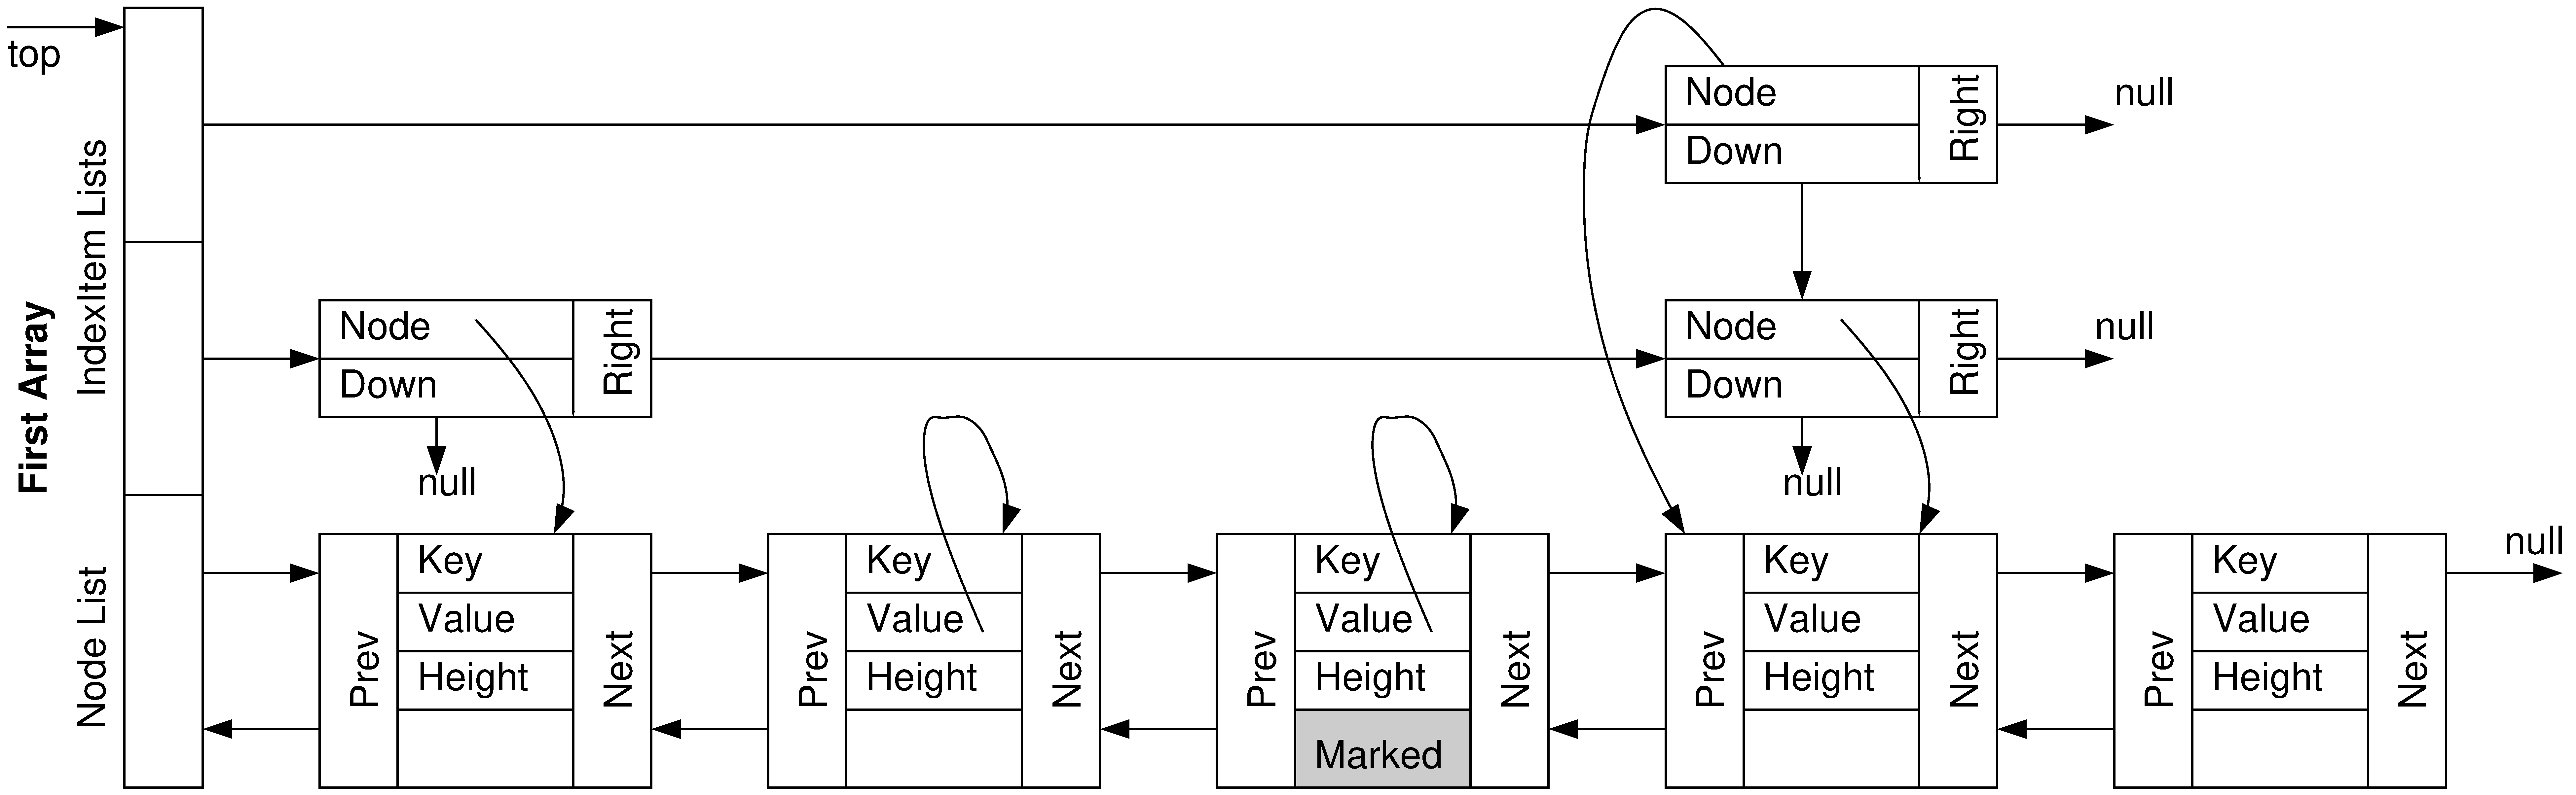
\includegraphics[scale=0.128]{Skip-list/fig/skiplist_diagram}
	\end{center}
	\caption{Skip list structure}
\end{figure*}


\subsection{Abstract operations}\label{ssec:abs}
% 
% The goal of these CF algorithms is for the abstract operations
%  to encounter and produce as little contention as possible.
% %
% In particular, it boils down to 
% %As previously discussed this means deletions are done by 
% setting the nodes
% $\ms{del}$ flag to $\lit{true}$ to delete a node 
% as well as linking 
% %insertions only insert 
% a new node to the bottom list level to insert it.
% These modifications are necessary to guarantee that
% linearizability, with other structural adaptations being saved for later execution.

The \opfont{contains}, \opfont{insert}, and \opfont{delete} operations start by traversing the towers using the \opfont{traverse-tower} procedure
that traverses the towers similar to a sequential skip list algorithm, moving forward in the list until reaching a node with a larger
key than $\ms{k}$ and then moving down a level.
If a node with key $\ms{k}$ is found then that node is returned immediately, otherwise the operations continues until the bottom of the tower is reached,
returning the node of the tower it stops at.

The traversal continues on the bottom list level using the \opfont{get-next-node} procedure.
The main differences between this traversal and a sequential algorithm is due to concurrent removals.
If a node is encountered in the list that has been marked to be removed (line \ref{lfline:get-helpcheck}) then
the \opfont{help-remove} procedure is called (line \ref{lfline:get-help}) or if a node is encountered that has already been
removed then the $\ms{prev}$ pointers are used to backtrack into the list.

During the \opfont{contains} operation, if a node with key $\ms{k}$ is found its value is read (lines \ref{lfline:con-eq1}-\ref{lfline:con-eq2}) and either $\lit{true}$ or $\lit{false}$ is returned depending on the observed value; if no node with key $k$ is found $\lit{false}$ is returned.

During a \opfont{delete} operation, if a node with key $\ms{k}$ is found that is neither removed
nor marked deleted (checked on line \ref{lfline:del-check}) then a \CAS{} is performed to try marking the node as deleted (line \ref{lfline:del-mod}).

An interesting implication of separating the structural adaptation is the ability 
to have lighter insertions.
An \opfont{insert} is executed ``logically'' if it encounters a node with key 
$\ms{k}$ that is marked
as deleted (lines \ref{lfline:ins-check}) by unmarking it (lines \ref{lfline:ins-mod}).
If no node with key $\ms{k}$ is found then the \opfont{insert} operation allocates ``physically'' a new 
node (line \ref{lfline:ins-addcall}) before
adding it to the list by performing a \CAS{} operation on the next pointer of the predecessor 
(line~\ref{lfline:ins-add1}).
Note that existing skip list algorithms cannot exploit logical insertions as each logical deletion is 
traditionally followed by a physical removal.
 

During both \opfont{insert} and \opfont{delete} operations if a \CAS{} operation fails (due to a concurrent modification) then the \opfont{get-next-node} procedure is called again,
starting the traversal from the node where the \CAS{} failed.


\subsection{Structural adaptation}\label{sec:adap}

The structural adaptation is executed repeatedly by a dedicated thread, called \emph{adapting thread}.
Its first task is to physically remove nodes marked as deleted
who have a height of $1$.
This is done after a successful \opfont{delete} operation, as well as in the adapting thread.
The \opfont{remove} operation is more difficult than the abstract operations as it requires three \CAS{} operations.
The reason is that a node cannot be safely removed from the list using just one \CAS{}.
Consider a node $\ms{n}$ to be removed that has predecessor and successor nodes $\ms{prev}$ and $\ms{next}$.
If a \CAS{} is performed on $\ms{prev.next}$ removing $\ms{node}$ by changing the pointer's value from $\ms{node}$ to $\ms{next}$ then
a concurrent \opfont{insert} operation could have added a new node in between $\ms{node}$ and $\ms{next}$, leading to a lost update problem~\cite{Val96}.
In order to avoid such cases, physical removals are broken into two steps.

First, the $\ms{v}$ field of the node to be removed is \CAS{}ed from $\bot$ to point to the node itself
on line \ref{lfline:rm-cas} of the \opfont{remove} operation.
This indicates to other threads that the node is going to be removed.
Then, the removal is completed in a separate \opfont{help-remove} procedure
(which might also be called by a concurrent operation performing a traversal).
%The reason for this is that since the removal takes several steps other threads might
%have to help with the removal in order that they are not blocked waiting for the removal to finish
%which would violate the non-blocking guarantee.

We encompass lost \opfont{insert} scenarios by using a special marked node, which is inserted with 
a \CAS{} just after the node to be removed (lines \ref{lfline:rm-marksetup1}-\ref{lfline:rm-marksetupcas}), 
similar to Lea's $\lit{ConcurrentSkipListMap}$.
%in order to prevent lost \opfont{insert} operations
%a marked node is allocated and \CAS{}ed to the list directly after the node to be removed (lines \ref{lfline:rm-marksetup1}-\ref{lfline:rm-marksetupcas}).
In order to distinguish a marked node from other nodes it has its $\ms{marked}$ flag set to $\lit{true}$ 
and its $\ms{v}$ field points to itself.
Additionally, a validation checks that neither the predecessor nor the successor node is marked 
before inserting a new node.
%During the \opfont{insert} operations, validation are done to prevent lost inserts by checking that 
%neither the
%predecessor nor the successor node is marked before inserting a new node
(lines~\ref{lfline:val-rem} and~\ref{lfline:val-check} of the~\opfont{get-next-node} procedure and on
line~\ref{lfline:ins-rmcheck} of the \opfont{insert} operation).
%Then, as soon as the node to be removed is found, 
%Once the marked node has been added to the list the predecessor of the node to be removed is
%found 
To complete the removal
a \CAS{} is performed on the predecessor's \opfont{next} pointer 
(line~\ref{lfline:rm-finalcas}) removing the node and its marker from the list.

A second task of the adapting thread is to
modify the upper levels of nodes in order to ensure
the $O(\log{n})$ expected traversal time.
Since neither removals nor insertions are done as they are in traditional skip lists,
calculating the height of a node must also be achieved differently.
Existing algorithms call a random function to calculate the heights of nodes,
here they are done deterministically while
considering that
the fundamental structure of a skip list is not designed
to be perfectly balanced (as it would be too costly) but rather probabilistically balanced.
This is done using the procedure \opfont{raise-index-level},
which is called at each tower level from the bottom level going upwards.
Each iteration traverses an entire list level, 
where each time it observes 3 consecutive nodes whose height equals this level (line~\ref{lfline:rl-check1}--\ref{lfline:rl-check2}),
it raises the level of the middle node by 1 (line~\ref{lfline:rl-raise2}).
%Starting from the bottom level going upwards, do the following at
%each level:
%Traverse the entire level.
%Each time $3$ nodes in a row of height equal to the current level
%are encountered, raise the level of the middle of these nodes by $1$.
Such a technique approximates the targeted number of nodes present at each level, 
balancing the structure.
%This creates an approximate correct number of nodes at each level
%and creates an approximately correct balance.

The final task of the adapting thread is due to the fact
that only towers of height 1 are physically removed
and is necessary in the case that ``too many'' tall nodes are marked as deleted.
If the number of nodes of levels greater than 1 that are logically deleted 
passes some threshold then
the \opfont{lower-index-level} procedure is called
 which removes the entire bottom $\ms{index-item}$ level of the skip list
by changing the $\ms{down}$ pointers of the level above to $\bot$ (line~\ref{lfline:ll-cas}).
Doing this avoids modification to the taller nodes in the list and helps ensure
there are not too many marked deleted nodes left in the list.
There are no frequent re-balancing going on to the tower, 
tall nodes will stay tall nodes meaning less contention
at the frequently traversed locations of the structure.

The adapting thread continually traverses the structure
repeating these structural adaptation procedures as necessary while also
physically removing appropriate nodes that were not
successfully removed by a \opfont{delete} operation.

\subsection{Non-Blocking}\label{ssec:progress}

In order for an algorithm to be considered non-blocking at least one thread must make progress after a sufficiently long
amount of time.
Since none of the operations use locks or any blocking operations the algorithm can be proven to be non-blocking
by showing that a thread can only be stuck infinitely in a loop if there is at least one other thread making progress.
Many of these loops traverse the skip list following the $\ms{next}$, $\ms{prev}$ pointers of the nodes or the $\ms{down}$,
$\ms{right}$ pointers of the IndexItems.
In Appendix~\ref{app:proof} we show that the skip list is valid which requires that nodes are sorted in ascending order by their keys.
Therefore these traversals can only loop infinitely if there is either an infinite number of nodes being added/removed from
the list concurrently.

First we will consider the while loop in the \opfont{get-next-index} procedure.
Iterations of this loop traverses forward and down levels of IndexItems.

The \opfont{help-remove} procedure has a while loop
on lines~\ref{lfline:rm-markcheck}--\ref{lfline:rm-next2}, this loop compares and swaps a marker node into the list, looping until a marker is added successfully.
In order for the addition of a marker node to fail an infinite number of times there must be an infinite number of concurrent successful
\opfont{insert} operations.

In the \opfont{get-next-node} procedure there is an inner while loop that traverses backward in the list (lines~\ref{lfline:get-while1s}--\ref{lfline:get-while1f})
and an outer level loop that traverses forward in the list (lines \ref{lfline:get-while2s}--\ref{lfline:get-while2f}).
An infinite traversal in the inner loop would require an infinite number of node removals which would also require and infinite
number of inserts.
An infinite number of outer loop iterations would require either a infinitely long list (which would mean an infinite number of inserts)
or an infinite number of invocations of the inner while loop.
The inner while loop is only invoked when the outer traversal reaches a node in the process of being removed.
Therefore in order for the inner loop to be invoked an infinite number of times
the outer traversal must encounter one or more marked removed nodes in the list an infinite number of times.
Each iteration of the outer loop calls the \opfont{help-remove} procedure, which
either successfully physically removes a node from the list or fails due to a concurrent operation succeeding.
If it succeeds an infinite number of times then there must be an infinite number of delete operations and if it fails an infinite number of times then
there must be an infinite number of concurrent operations modifying the list structure (be it inserts or removals), in either case at least one other thread is making progress.

Both the \opfont{insert} and \opfont{delete} operations contain a while loop.
In both operations an iteration of the while loop will always exit unless it calls a \CAS{} that fails.
Both operations might perform a \CAS{} on the $\ms{v}$ field of a node (line~\ref{lfline:ins-mod} of \opfont{insert} and line~\ref{lfline:del-mod}  of \opfont{delete}),
but this \CAS{} will only fail due to a concurrent \opfont{insert} or \opfont{delete} successfully performing a \CAS{} on this field.
The \opfont{insert} operation might perform a \CAS{} on line~\ref{lfline:ins-add1} changing a node's pointer, this \CAS{} can only fail
due to a concurrent successful insert or removal.
Therefore an infinite loop in these operations is only possible due to infinite number of successful operations by at least one other thread.

\subsection{Garbage collection}\label{ssec:gc}

Nodes that are physically removed from the data structures must be garbage collected.
Once a node is physically removed it will no longer be reachable by future operations.

Concurrent traversal operations could be preempted on a removed node so 
the node cannot be freed immediately.
In languages with automatic garbage collection these nodes will be freed as soon 
as all preempted traversals continue past this node.
If automatic garbage collection is not available then some additional mechanisms can be used.
One possibility is to provide each thread with a local operation counter and a boolean 
indicating if the tread is currently performing an abstract operation or not.
Then any physically removed node can be safely freed as long as each thread is either not performing an abstract operation or if it has increased its counter since the node was removed.
This can be done by the adapting thread.
Other garbage collection techniques can be used such as reference counting described in~\cite{DMM+01}.

% \subsection{Distributed structural adaptation}\label{sec:disMaint}
% Each structural adaption is a short local operation, yet each round of structural adaptation is done by a 
% complete traversal
% of the data structure.
% Some might argue that if all the hardware of a system is already in use by program threads then why not 
% break the structural adaptation into smaller structural adaptations and distribute them over the abstract 
% modifications. The reason for not doing this is twofold.
% 
% Firstly even though each structural adaption is a very local operation, they use global information.
% Since only nodes with height $1$ are removed from the skip list the structural adaptation needs to know 
% about the heights
% of the other nodes before raising the level of a node in order to ensure that the structure does not 
% become unbalanced.
% Before resizing the hash table the structural adaptation should know approximately how many nodes 
% are in the table.
% 
% Secondly the structural adaptations are in some cases more costly (in terms of computation, not 
% contention) then in existing data structures.
% For example choosing the levels of nodes in the skip list requires previously traversing the other 
% nodes to know their height.


\begin{figure*}
	\begin{center}
	\subfigure[Tolerance to contention of the non-blocking skip lists\label{fig:cf}]{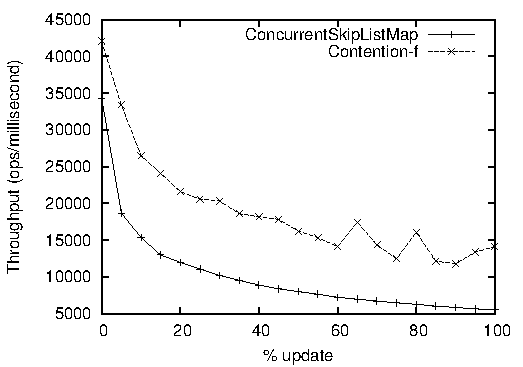
\includegraphics[scale=0.8]{Skip-list/experiments/tyler/update_main_77}}
	\subfigure[Scalability of the non-blocking skip lists\label{fig:scalability}]{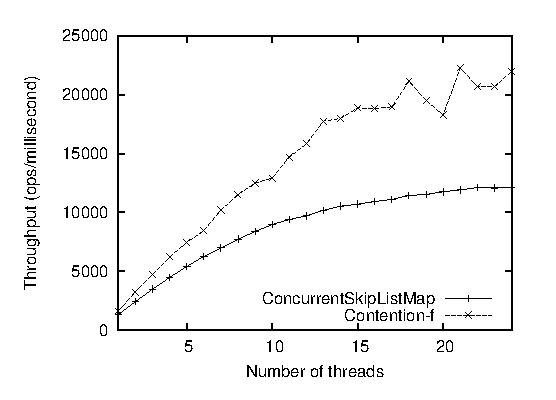
\includegraphics[scale=0.8]{Skip-list/experiments/tyler/cores_main_76}}
	\end{center}
	\caption{Comparison of our contention-friendly non-blocking skip list against the JDK concurrent skip list (ConcurrentSkipListMap)}
\end{figure*}




\subsection{Distributing the structural adaptation}\label{ssec:distrib}

%\vincent{I moved the motivations for having a single adapting thread from the CF section to this part and I mentioned that we only use one thread for it in the algorithm section, not in the CF section.
%The goal here is to say that we give the feeling that we could do the structural adaptation on multiple threads (distributed) but that it complexifies the algorithm and presents some drawbacks.}

The algorithm we have presented exploits the multiple computational resources available on 
today's multicore machines by having a separate adapting thread. 
It could be adapted to support multiple adapting threads or to make each application thread participate 
into a distributed structural adaptation (if for example computational resources get limited). 
Although this 
approach is appealing to, for example, to maintain the big-oh complexity despite failures, it makes the protocol more 
complex.

To keep the benefit from the contention-friendliness of the 
protocol, it is important to maintain the decoupling between the abstract 
modifications and the structural adaptations. 
Distributing the tasks of the adapting thread to each application threads should not force them to  
execute a structural adaptation systematically after each abstract modification.
Instead, each application thread could toss a coin after each of its 
abstract modification to decide whether to run a structural adaptation.
This raises an interesting question on the optimal proportion of abstract 
modifications per adaptation.

%Each structural adaption is a short local operation, yet each round of structural adaptation is done by 
%a complete traversal of the data structure.
%Some might argue that if all the hardware of a system is already in use by program threads then 
%why not break the structural adaptation
%into smaller structural adaptations and distribute them over the abstract modifications.
%The reason for not doing this is twofold.

The other challenge is to guarantee that concurrent structural adaptations execute safely.
This boils down into synchronizing the higher levels of the skip list by using \CAS{}
each time a pointer of the high level lists is adapted. 
An important note is that given the probability distribution of nodes per level in the skip list, the sum 
of the items in the upper list levels is approximately equal to the number of nodes in the bottom 
list level. On average the amount of conflicts induced by the skip list with a distributed adaptation 
could be potentially twice the one of the centralized adaptation. This exact factor depends, 
however, on the frequency of the distributed structural adaptation.
%On average the amount of conflicts created by the contention friendly skip list is similar to that
%of a simple concurrent linked list, while a traditional concurrent skip list creates up to twice as 
%much contention.

Finally, to distribute the structural adaptation each thread could no longer rely on the global 
information regarding the heights of other nodes. To recover to the probability distribution of item to 
levels without heavy inter-threads synchronization, a solution would be to give up the 
deterministic level computation adopted in the centralized version and to switch back 
to the traditional probabilistic technique: each application thread inserting a new node would 
simply choose a level $\ell$ with probability $2^{-O(\ell)}$.

%Also since the thread takes care of choosing the height of all nodes, it can choose the height of a node 
%based on the height and location of the rest of the nodes instead of relying on a random function.

%Firstly even though each structural adaption is a very local operation, they use global information.
%%For example rotations in a tree need balance information that is propagated from the leaves.
%%Since only nodes with height $1$ are removed from the skip list the structural adaptation needs to know about the heights
%of the other nodes before raising the level of a node in order to ensure that the structure does not become unbalanced.
%Before resizing the hash table the structural adaptation should know approximately how many nodes are in the table.

%Secondly the structural adaptations are in some cases more costly (in terms of computation, not contention) then in existing data structures.
%For example a rotation requires allocating a new node, choosing the levels of nodes in the skip list
%requires previously traversing the other nodes to know their height, and resizing the hash table first requires
%counting the nodes.
%
%Such algorithms with distributed structural adaptation might be possible, but have not been examined here, but could be
%interesting to study in the future.

%\paragraph{Maintenance thread}
%Given that only nodes of height 1 are physically removed and the insert operations contains no structural adaptation
%then the ``maintenance'' thread is the only thread modifying the upper list levels.
%Therefore the ``maintenance'' thread will be the only thread making modifications to the upper list level so it can do it
%using simple reads and writes instead of using more costly synchronization mechanisms such as locks.
%Conflicts between any operations only occur on the bottom list level.
%Taking the probability distribution of nodes per level in the skip list into account, the sum of the items in the upper list
%levels is approximately equal to the number of nodes in the bottom list level.
%Therefore one could consider that on average the amount of conflicts created by the contention friendly skip list is similar to that
%of a simple concurrent linked list, while a traditional concurrent skip list creates up to twice as much contention.

%\paragraph{Why being centralized?}
%By performing the structural adaptation in a single thread means that there is no contention between 
%concurrent insert operations at the upper list levels so upper level can be modified using reads and 
%writes instead of \CAS{} or locks.
%Also since the thread takes care of choosing the height of all nodes, it can choose the height of a node 
%based on the height and location of the rest of the nodes instead of relying on a random function.
%A final advantage is that since these data structures are designed for architectures that use many cores
%performing the structural adaptation on a dedicated separate thread takes advantage of 
%hardware that might otherwise be left idle.

\section{Evaluation}\label{sec:expe}
Here we compare our skip list to the \opfont{java.util.concurrent} skip list on a multi-core machine. 
Additional experiments are deferred to Appendix~\ref{app:expe}.
%In short, this evaluation indicates that (i)~starvation is sufficiently rare in practice to be non-observable 
%even under high contention and (ii)~contention-friendliness allows to speed up the performance of 
%the mostly deployed concurrent skip list by a multiplying factor of $1.4$. (Additional experiments are 
%deferred to Appendix~\ref{app:expe}.)
%\paragraph{Settings.}
The machine is an AMD with two 12-core processors, comprising 24 hardware threads 
in total. For each run we averaged the number of
executed operations per millisecond over 5 runs of 5 seconds. 
Thread counts are from $1$ to $24$ and the five runs execute 
successively as part the same JVM for the sake of warmup.
We used Java SE 1.6.0 12-ea in server mode and HotSpot JVM 11.2-b01.

The approximate number of elements in the set abstraction is 5 thousand with
operations choosing from a range of 10 thousand keys, implying that each update 
operation successfully modify the data structure 50\% of the time. As insertions and deletions
are executed with the same probability the data structure size remains constant in expectation.

The \opfont{ConcurrentSkipListMap} is Doug Lea's Java implementation 
relying on Harris, Michael and Fraser algorithms~\cite{Har01,Mic02,Fra03}.
It comes with JDK 1.6 as part of the \opfont{java.util.concurrent} package.
We compare this implementation to our contention-friendly skip list as  given in 
Section~\ref{sec:datastruct}---both implementations are non-blocking.

%We compare the following algorithms
%\begin{itemize}
%\item {\bf ConcurrentSkipListMap:} This algorithm is Doug Lea's Java based non-blocking skip list
%$\lit{ConcurrentSkipListMap}$ relying on Harris and Michael algorithms~\cite{Har01,Mic02}.
%\item {\bf Contention-friendly version:} This algorithm (Contention-f) uses the contention friendly 
%methodology.
%There is a dedicated thread that takes care of all modifications to the upper list levels as well as 
%physical removals.
%The program threads do not modify the upper list levels, only performing inserts and deletes to the 
%bottom level
%as well as physical removals.
%\end{itemize}

%\paragraph{Results.}
Figure~\ref{fig:cf} depicts the tolerance to contention of the algorithms, by increasing the percent of 
update operations from 0 to 100 (i.e., between 0\% and 50\% effective structure updates).
We can see that the contention-friendly (Contention-f) skip list better tolerates contention than the 
\opfont{ConcurrentSkipListMap} which results in significantly higher performance.

An interesting result is the gain of using our skip list at 0\% update: since the contention-friendly
skip list tolerates high contention, it can afford maintaining indices for half of the nodes, so that 
half of the node have multiple levels. In contrast,  \opfont{ConcurrentSkipListMap} maintains the 
structure so that only one quarter of the nodes have indices, in an attempt
to reduce the contention when updates come into play. Actually, our strategy better tolerates
contention when updates appear as the contention-friendly skip list is up 
to $2.5\times$ faster than the \opfont{ConcurrentSkipListMap}.
%In particular, although the contention-friendly skip list is more efficient as 0\% update 
%the most important performance gain is between 
%5\% and 45\% of updates. 
%At higher update ratios, the contention becomes high yet the contention-friendly structure provides significantly higher throughput than the \opfont{ConcurrentSkipListMap} version.

Figure~\ref{fig:scalability} compares the performance of the skip list algorithms, run with 20\% of 
update operations (i.e., 10\% effective structure updates). 
Although the \opfont{ConcurrentSkipListMap} scales well with the number of threads, the contention-friendly skip list scales better. In fact, the decoupling of the later allows to tolerate the contention raise 
induced by the growing amount of threads, leading to a performance speedup of up to $1.8\times$.
%The contention-friendly skip list scales better 
%than the \opfont{ConcurrentSkipListMap} with the number of threads. In fact, it exploits the concurrency
%by tolerating the contention raise induced by the growing amount of threads. Although the \opfont{ConcurrentSkipListMap} scales well, its tied structural adaptation is costly and induces additional 
%overhead when compared to the decoupled one.


%with $2^{14}$ (left) and 
%$2^{16}$ elements (right) and on a read-only workload (top) and workloads comprising up to 30\% 
%updates (bottom).
%While all data structures scale well with the number of threads, the $\lit{ConcurrentSkipListMap}$ is 
%slower then its contention-friendly counterparts in all the various settings.

%Finally Appendix~\ref{sec:tm} shows that our adaptation of the CF methodology to transactional
%memory algorithms allows a performance benefit of $1.5\times$ on average.

%\begin{figure}
%\includegraphics[scale=1.0]{experiments/new/pdf/update-lf45}
%\vspace{-1em}
%\caption{\footnotesize{Tolerance to contention of various non-blocking skip lists\label{fig:scalability}}}
%\end{figure}

%\begin{table*}
%\begin{center}
%{\footnotesize
%\renewcommand{\tabcolsep}{1pt}
%\renewcommand{\arraystretch}{1}
%\begin{tabular}{|c|c|c|}
%	\hline
%	Data structures & non-CF variant & Description \\ \hline\hline
%	Hash table & ConcurrentHashMap & Lock-based hash table of the \texttt{java.util.concurrent} package \\ \hline
%	Search tree & Optimistic tree & A practical binary search tree using optimistic concurrency control \cite{BCCO10} \\ \hline
%	Skip list & ConcurrentSkipList & Doug Lea's implementation with logical 
%	deletion~\cite{Har01,Mic02} \\ \hline
%\end{tabular}
%}
%\caption{\footnotesize Non Contention-Friendly Data Structures\label{table:non-cf-ds}}
%\end{center}
%\end{table*}

%
%Figure~\ref{fig:updates} depicts the tolerance to contention of the algorithms.
%More precisely, it indicates the slowdown of each algorithms under contention as the normalized 
%ratio of its performance with non-null update ratios over its performance without updates.
%The slowdown of non-CF skip list always more significant than the one of their CF counterpart, 
%indicating that the CF is more tolerant to contention.
%%
%\begin{floatingfigure}{9cm}
%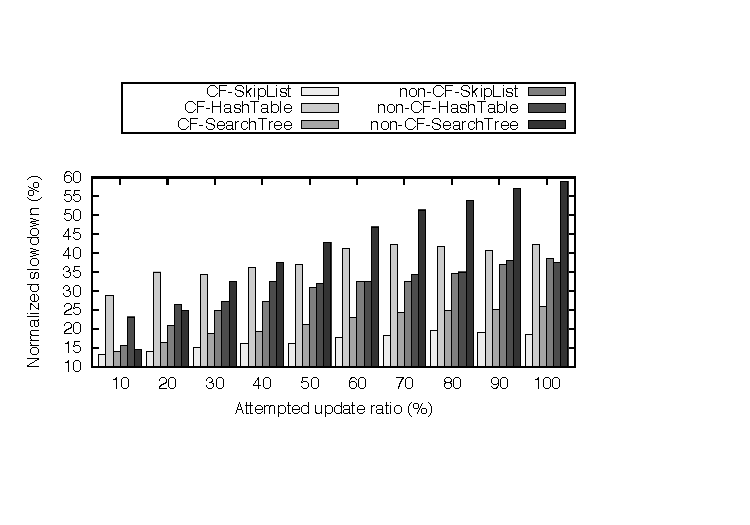
\includegraphics[scale=0.9,clip=true,viewport=10 50 280 230]{experiments/old/pdf/updates}
%\vspace{-1em}
%\caption{\footnotesize{Tolerance to contention of Contention-Friendly (CF) and non-CF algorithms (performance slowdown with respect to 0\% updates)\label{fig:updates}}}
%\end{floatingfigure}
%%
%
%Figure~\ref{fig:perf} compares the performance of the same algorithms with $2^{14}$ (left) and $2^{16}$ elements (right) and on a read-only workload (top) and workloads comprising up to 30\% updates (bottom).
%While all data structures scale well with the number of threads, the $\lit{ConcurrentSkipListMap}$ is slower then its contention-friendly counterparts in all the various settings.
%
%Finally Appendix~\ref{sec:tm} shows that our adaptation of the CF methodology to transactional memory algorithms allows a performance benefit of $1.5\times$ on average.
%
%\begin{figure}
%\begin{center}
%\subfigure[$2^{14}$ elements\label{fig:214}]{\includegraphics[scale=0.45,clip=true,viewport=55 60 555 800]{experiments/old/pdf/raw-perf-16384-60}}\hspace{0.5em}
%%\caption{Performance of the Contention-Friendly (CF) and non-CF data structures with $2^{14}$ elements\label{fig:perf}}
%%%%%%%%%%%%%%%%%%%%%%%%%%%%%%%%%%
%%TECH_REPORT
%\iftoggle{tech_report} {
%\end{center}
%\end{figure}
%\begin{figure}
%\begin{center}
%%%%%%%%%%%%%%%%%%%%%%%%%%%%%%%%%%
%%end toggle TECH_REPORT
%}{}
%\subfigure[$2^{16}$ elements\label{fig:216}]{\includegraphics[scale=0.45,clip=true,viewport=97 60 555 800]{experiments/old/pdf/raw-perf-65536-60}}
%%\caption{Performance of the Contention-Friendly (CF) and non-CF data structures with $2^{16}$ elements\label{fig:perf}}
%\caption{Performance of the Contention-Friendly (CF) and non-CF data structures\label{fig:perf}}
%\end{center}
%\end{figure}



%\begin{figure}
%\begin{center}
%\includegraphics[scale=0.38]{experiments/pdf/raw-perf-16384-60}
%\caption{Performance of the Contention-Friendly (CF) and non-CF data structures with $2^{14}$ elements\label{fig:perf}}
%\end{center}
%\end{figure}
%
%\begin{figure}
%\begin{center}
%\includegraphics[scale=0.38]{experiments/pdf/raw-perf-65536-60}
%\caption{Performance of the Contention-Friendly (CF) and non-CF data structures with $2^{16}$ elements\label{fig:perf}}
%\end{center}
%\end{figure}



\section{Conclusion}\label{sec:conclusion}

Multicore programming brings new challenges, like contention, that programmers have to anticipate
when developing every day applications.
%Programmers should now think carefully about contention overhead
%in addition to big-oh complexity.
We explore the design of a contention-friendly and non-blocking skip list, keeping in 
mind that contention
is an important cause of performance drop.
%We explored the methodology of designing a contention-friendly skip list, keeping in mind that contention will be a predominant cause of performance loss in tomorrow's architectures.
%This simple methodology led to a novel Java package of concurrent data structures more efficient than the best implementations we could find.
As future work, we would like to derive new contention-friendly data structures.



% 
% \bibliographystyle{abbrv}
% \bibliography{bib}
% 
% \begin{appendix}




\section{Additional Evaluation}\label{app:expe}


\begin{figure*}\label{fig:smallUp}
	\begin{center}
 	\subfigure[Throughput, range of 128 elements\label{fig:smallTp}]{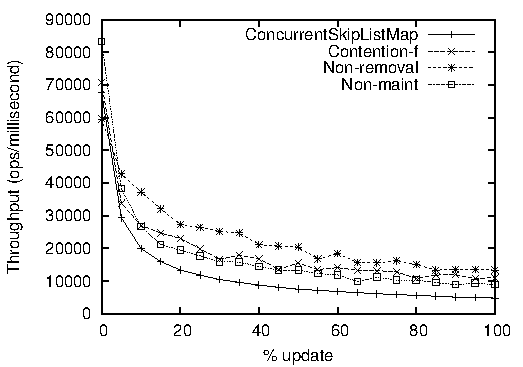
\includegraphics[scale=0.8]{Skip-list/experiments/tyler/update_Update0largerange_70_small}}
 	\subfigure[Slowdown, range of 128 elements\label{fig:smallSd}]{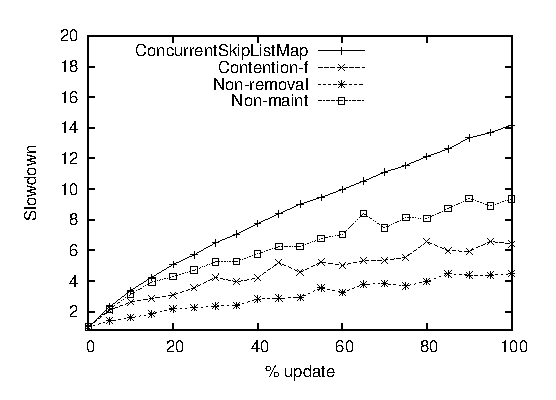
\includegraphics[scale=0.8]{Skip-list/experiments/tyler/update_slowdown_Update0largerange_70_small}}
 	\subfigure[Throughput, range of 128k elements\label{fig:smallTpLr}]{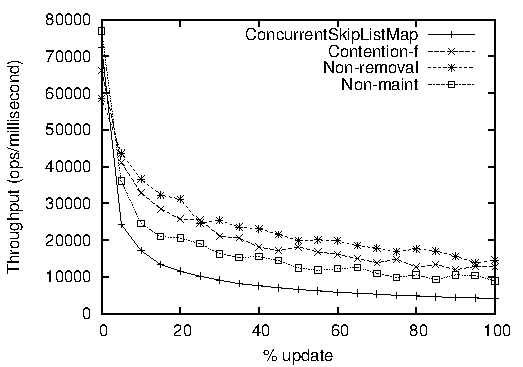
\includegraphics[scale=0.8]{Skip-list/experiments/tyler/update_Update50largerange_71_small}}
 	\subfigure[Slowdown, range of 128k elements\label{fig:smallSdLr}]{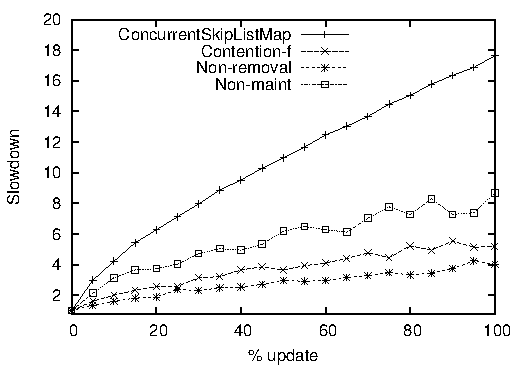
\includegraphics[scale=0.8]{Skip-list/experiments/tyler/update_slowdown_Update50largerange_71_small}}
	\end{center}
	\caption{Comparison of \% update ratio using our non-blocking skip lists against the JDK concurrent skip list (ConcurrentSkipListMap) using a set of size 64 elements}
\end{figure*}


\begin{figure*}\label{fig:largeUp}
	\begin{center}
 	\subfigure[Throughput, range of 128k elements\label{fig:largeTp}]{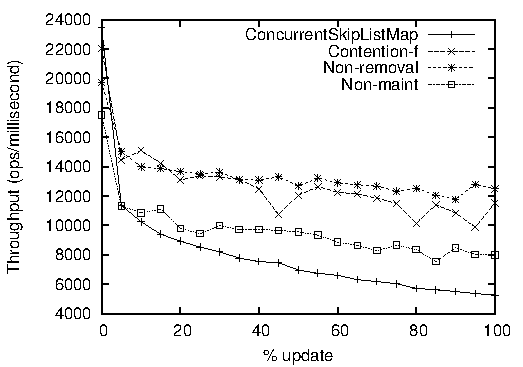
\includegraphics[scale=0.8]{Skip-list/experiments/tyler/update_Update0largerange_70_large}}
 	\subfigure[Slowdown, range of 128k elements\label{fig:largeSd}]{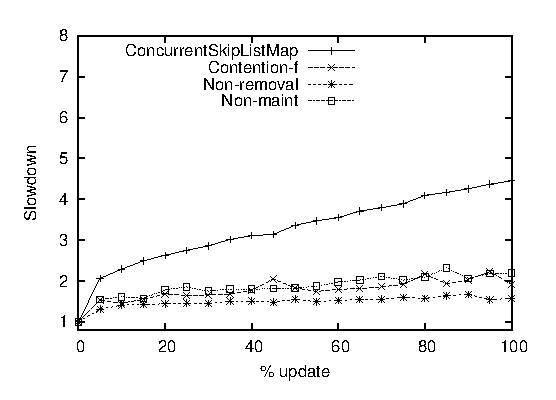
\includegraphics[scale=0.8]{Skip-list/experiments/tyler/update_slowdown_Update0largerange_70_large}}
 	\subfigure[Throughput, range of 128 million elements\label{fig:largeTpLr}]{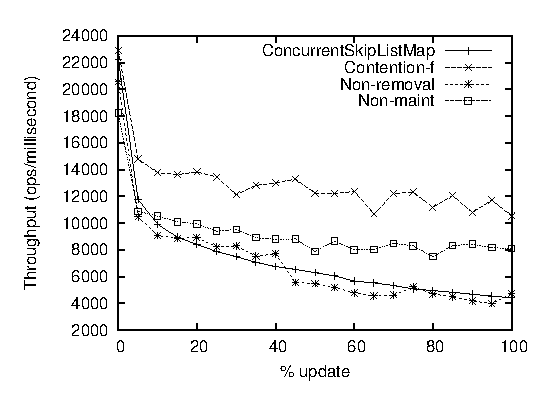
\includegraphics[scale=0.8]{Skip-list/experiments/tyler/update_Update50largerange_71_large}}
 	\subfigure[Slowdown, range of 128 million elements\label{fig:largeSdLr}]{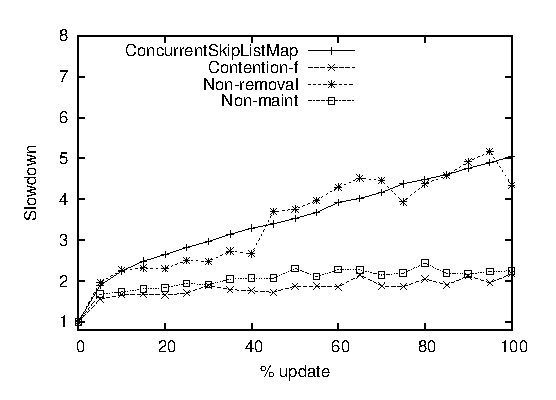
\includegraphics[scale=0.8]{Skip-list/experiments/tyler/update_slowdown_Update50largerange_71_large}}
	\end{center}
	\caption{Comparison of \% update ratio using our non-blocking skip lists against the JDK concurrent skip list (ConcurrentSkipListMap) using a set of size 64k elements}
\end{figure*}


\begin{figure*}\label{fig:smallThd}
	\begin{center}
 	\subfigure[10\% update, range of 128 elements\label{fig:smallTd10}]{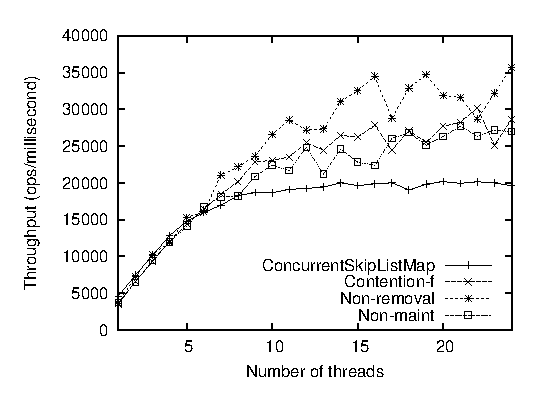
\includegraphics[scale=0.8]{Skip-list/experiments/tyler/cores_10update0largerange_60_small}}
 	\subfigure[100\% update, range of 128 elements\label{fig:smallTd100}]{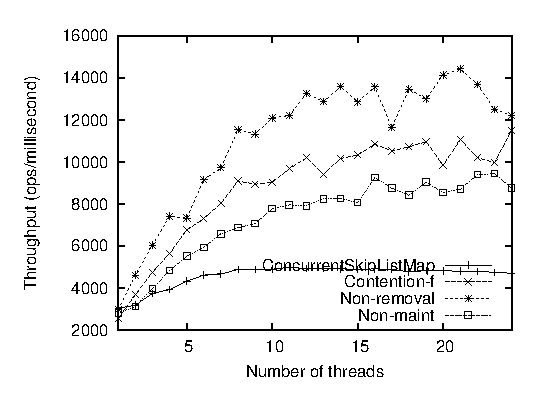
\includegraphics[scale=0.8]{Skip-list/experiments/tyler/cores_100update0largerange_72_small}}
 	\subfigure[10\% update, range of 128k elements\label{fig:smallTdLr10}]{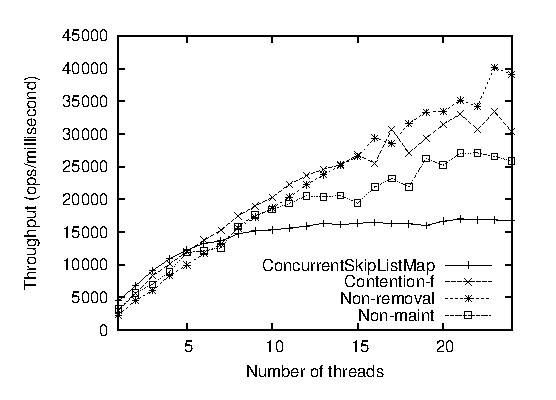
\includegraphics[scale=0.8]{Skip-list/experiments/tyler/cores_10update50largerange_63_small}}
 	\subfigure[100\% update, range of 128k elements\label{fig:smallTdLr100}]{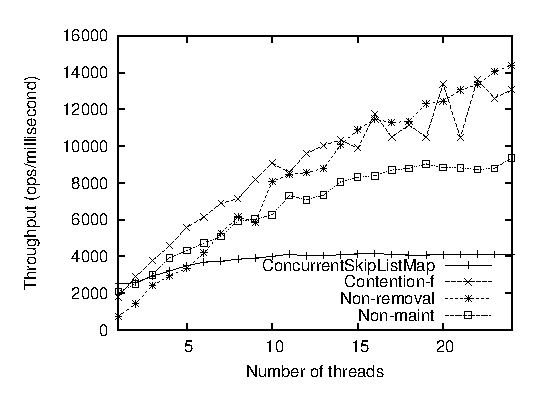
\includegraphics[scale=0.8]{Skip-list/experiments/tyler/cores_100update50largerange_64_small}}
	\end{center}
	\caption{Comparison of number of threads using our non-blocking skip lists against the JDK concurrent skip list (ConcurrentSkipListMap) using a set of size 64 elements}
\end{figure*}


\begin{figure*}\label{fig:largeThd}
	\begin{center}
 	\subfigure[10\% update, range of 128k elements\label{fig:largeTd10}]{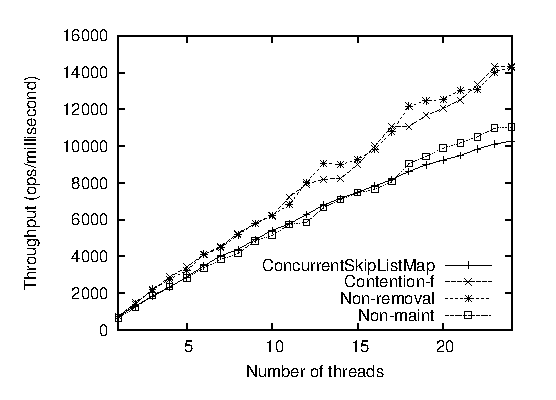
\includegraphics[scale=0.8]{Skip-list/experiments/tyler/cores_10update0largerange_60_large}}
 	\subfigure[100\% update, range of 128k elements\label{fig:largeTd100}]{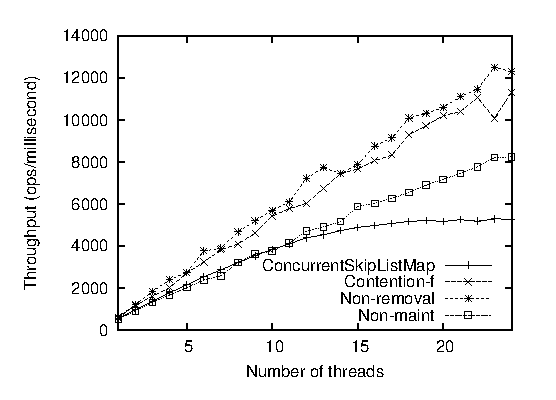
\includegraphics[scale=0.8]{Skip-list/experiments/tyler/cores_100update0largerange_72_large}}
 	\subfigure[10\% update, range of 128 million elements\label{fig:largeTdLr10}]{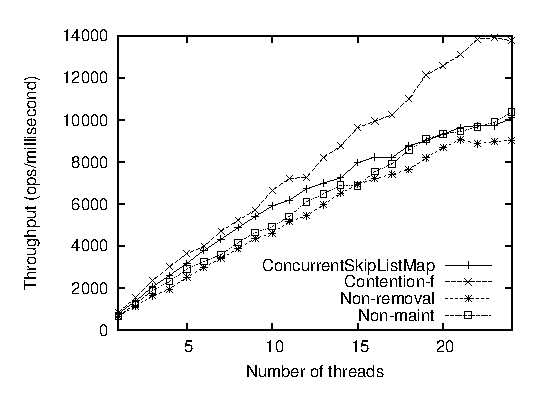
\includegraphics[scale=0.8]{Skip-list/experiments/tyler/cores_10update50largerange_63_large}}
 	\subfigure[100\% update, range of 128 million elements\label{fig:largeTdLr100}]{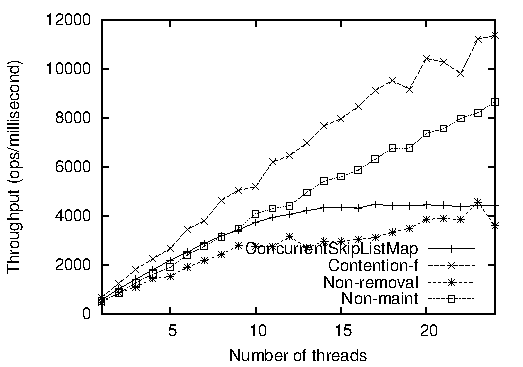
\includegraphics[scale=0.8]{Skip-list/experiments/tyler/cores_100update50largerange_64_large}}
	\end{center}
	\caption{Comparison of number of threads using our non-blocking skip lists against the JDK concurrent skip list (ConcurrentSkipListMap) using a set of size 64k elements}
\end{figure*}



\begin{figure*}\label{fig:growShrink}
	\begin{center}
 	\subfigure[Grow benchmark\label{fig:grow}]{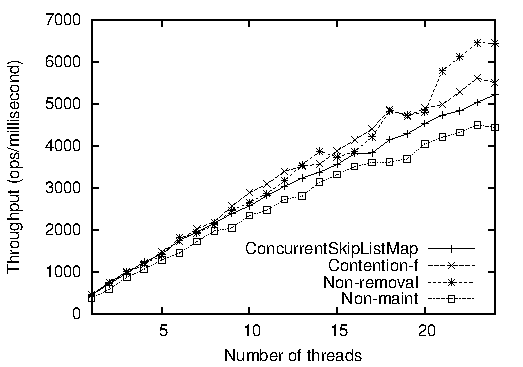
\includegraphics[scale=0.8]{Skip-list/experiments/tyler/cores_Grow_74}}
 	\subfigure[Shrink benchmark\label{fig:shrink}]{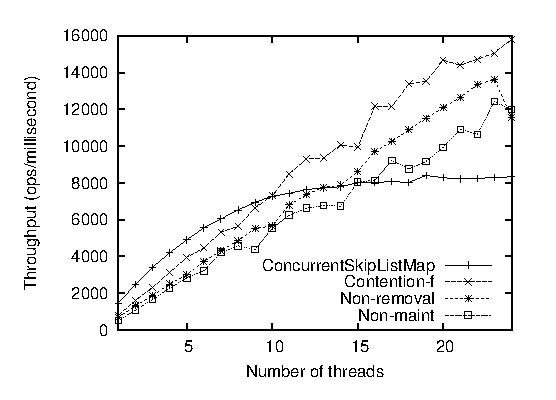
\includegraphics[scale=0.8]{Skip-list/experiments/tyler/cores_Shrink_73}}
	\end{center}
	\caption{Comparison of number of threads using our non-blocking skip lists against the JDK concurrent skip list (ConcurrentSkipListMap) using the grow and shrink benchmark}
\end{figure*}


In this section we present additional performance results.
Each benchmark was run 4 times (the average of the 4 runs is presented in the figures) each with a duration of 5 seconds with the JVM being warmed up for 5 seconds prior to running each benchmark.
In order to better understand where the benefits of the contention friendly algorithm are coming from
we present two additional variations of the algorithm:
\begin{itemize}
\item {\bf Non-removal contention-friendly version:} This version of the algorithm (Non-removal) does not perform any physical removals.
A node that is deleted is marked as deleted, but stays in the skip list forever.
This algorithm helps us examine the cost of contention caused by physical removals.
A dedicated maintenance thread that takes care of 
modifications to the upper list levels. 
\item {\bf Non-maintenance contention-friendly version:} This version of the algorithm (Non-maint) has no dedicated maintenance thread.
It only uses the selective removals concept of contention friendliness; only nodes of height 1 are physically removed.
This version helps us examine the benefits of using a maintenance thread.
Given that there is no maintenance thread, modifications to the upper list levels are done as part of the abstract operations.
A node's height, like in a traditional skip list, is chosen during the \opfont{insert} operation by a random function with the one exception
that a height greater than 1 will only be chosen
if both node's neighbors have a height of 1.
This helps prevent there from being ``too many'' tall nodes due to the fact that only nodes of height 1 are physically removed.
\end{itemize}


Figure \ref{fig:smallTp}-\ref{fig:smallSdLr} compares the effect of increasing the amount of update operations on the algorithms.
The update ratio start at 0\% and is increased to 100\% (50\% effective).
The set contains approximately 64 elements throughout the benchmarks with small variations due to concurrency.
The range of elements the abstract operations can choose from is either 128 or 128 thousand.
The smaller range allows for higher contention on specific keys in the set while the larger range allows for more
variation in the keys in the set.
The graphs show both higher performance and less slowdown of the contention friendly algorithms compared to $\lit{ConcurrentSkipListMap}$.
Between the contention-friendly versions we see that $\lit{Non-removal}$ provides the best performance.
This can be explained by the fact that since the size of the set is so small performing marked removals is much less contention-effective
than physically removing nodes.

Figure \ref{fig:largeTp}-\ref{fig:largeSdLr} is the same benchmark as Figure \ref{fig:smallTp}-\ref{fig:smallSdLr} except it is run with a set size of approximately 64 thousand elements
using ranges of 128 thousand and 128 million.
$\lit{Contention-f}$ shows both good performance and small slowdown while $\lit{Non-maint}$ shows performance in-between $\lit{Contention-f}$ and
$\lit{ConcurrentSkipListMap}$.
$\lit{Non-removal}$ shows the best performance with the range of 128 thousand elements, but performs poorly when the range is set to 128 million elements.
Since the range is so large and $\lit{Non-removal}$ does not perform any physical removals the number of marked deleted nodes in the skip list grows
so large that the cost of traversal becomes more expensive than in the other algorithms.
In this benchmark we see the number of nodes in the skip list to be as large as 6 million.


Figure \ref{fig:smallTd10}-\ref{fig:smallTdLr100} tests the scalability of the algorithms by showing the effect of increasing the number of threads from 1 to 24.
The tests were done with a 10\% and 100\% update ratios with a set size of 
approximately 64 elements.
Here we see better scalability from the contention-friendly algorithms compared to the 
$\lit{ConcurrentSkipListMap}$.
$\lit{Non-removal}$ shows in general the best performance due to the reduced contention from not doing physical removals (thanks especially to the small set size),
followed by $\lit{Contention-f}$, $\lit{Non-maint}$, and finally $\lit{ConcurrentSkipListMap}$.

Figure \ref{fig:largeTd10}-\ref{fig:largeTdLr100} also tests the scalability of the algorithms and is the same benchmark as \ref{fig:smallTd10}-\ref{fig:smallTdLr100} except it is run with a set size of approximately 64 thousand elements
using ranges of 128 thousand and 128 million.
At 10\% update all algorithms show good scalability, while at 100\% updates $\lit{ConcurrentSkipListMap}$ does not scale as well, with $\lit{non-removal}$ scaling the worst in
the larger range benchmark due to it not physically removing nodes.
In general $\lit{Contention-f}$ is the best performer followed by $\lit{Non-maint}$.

The purpose of figure \ref{fig:grow}-\ref{fig:shrink} is to test the scalability of the algorithms when the number of elements in the set changes by a large amount.
In the grow benchmark the size of the set starts at 0 elements and grows until a size of 500 thousand elements, while the shrink benchmark starts with
a set of size 500 thousand elements and ends with 2,500 elements.
Both benchmarks are executed with a 50\% update ratio.
All algorithms show good scalability in the grow benchmark with a small performance advantage going to the algorithms with maintenance threads ($\lit{Contention-f,Non-removal}$)
thanks to not requiring synchronization operations to the towers.
In the shrink benchmark we see that the $\lit{ConcurrentSkipListMap}$ performs best at small thread counts while the contention-friendly algorithms show better scalability.
Due to the decreasing list size $\lit{Contention-f}$ calls the \opfont{lower-index-level} procedure on average 4 times per run of the benchmark and at the end of the
benchmark the skip list contains around 15 thousand marked deleted nodes.
\opfont{lower-index-level} is called by the maintenance thread when it discovers that there are at least 10 times more marked deleted nodes than non-marked deleted ones.
This number can be tuned so that the procedure is called more often.



\section{Correctness}\label{app:proof}

Here we show that the CF non-blocking skip list implements a map
that is linearizable~\cite{HW90}.
The proof is separated into two parts, first we show that performing
\opfont{contains}, \opfont{insert}, and \opfont{delete} always results in a \emph{valid} skip list structure.
Second we show that each operation has a linearization point.

\paragraph{Definitions.} 
The skip list presented here represents the set (or map) abstract data type.
A key $\ms{k}$ is in the set if there is a path from the field $\ms{top}$ to a node with 
key equal to $\ms{k}$ with a non-$\bot$ value,
otherwise it is not in the set.
Therefore a \emph{valid} skip list has the following properties:
(i) the nodes in the skip list are sorted by their keys in ascending order,
(ii) there is a path from the field $\ms{top}$ to at most one node with a key $\ms{k}$ at any point in time 
and
(iii) every node with value $\ms{v \neq node}$ has a path to it from $\ms{top}$.
We consider that an operation \opfont{contains}, \opfont{insert}, and \opfont{delete} is a \emph{success} if it returns $\lit{true}$, otherwise it \emph{fails}.

For the sake of simplicity the structure is initialized with a single node with key $- \infty$ and a tower of maximum height.
Each of the IndexItems of the tower have their $\ms{right}$ pointer initialized to $\bot$ and the node's $\ms{next}$ pointer is also
initialized to $\bot$.


Before we define the linearization points of the operations we need the following two lemmas.

\begin{lemma}
\label{lemma:inlistlf}
If a node $\ms{n}$ is such that $\ms{n.next} = n'$ where $\ms{n'.marker} = \lit{true}$ and $\ms{n.value} = n$
then there is no longer a path from $\ms{top}$ to $\ms{n}$.
%
%A node (that at one point had a path to it from $\ms{top}$) no longer has a path to it from $\ms{top}$ only if the node's $\ms{next}$ pointer points to a marker node
%and the node's value is a pointer to itself.
\end{lemma}
\begin{proof}[Proof sketch]
Nodes are only unlinked from the list during a \opfont{help-remove} operation.
To prove the lemma it needs to be shown that the only two nodes unlinked from the list are $\ms{node}$ and the marker node that follows it in the list.
The CAS on line \ref{lfline:rm-finalcas} ensure that there
are no nodes in between $\ms{node}$ and its predecessor.
Lines \ref{lfline:rm-marksetup1}-\ref{lfline:rm-marksetupcas} CAS exactly one marker node after $\ms{node}$.
To show that no nodes are added before or after the marker node we will show that pointers to and from marker nodes are never modified
by considering all locations where the structure of the list is modified.
First we consider the places where a new node can be added to the list.
There are two places were a new node can be added to the list, this is on line \ref{lfline:rm-marksetupcas} of the \opfont{help-remove} procedure
and line \ref{lfline:ins-add1} of the \opfont{insert} operation.
In the case of the \opfont{help-remove} procedure, before adding a new marker node
it checks that the predecessor and the successor nodes are not markers (line \ref{lfline:rm-rmhelpcheck} and \ref{lfline:rm-markcheck}).
The same is done during the \opfont{insert} operation on lines \ref{lfline:val-rem} and \ref{lfline:val-check} of \opfont{get-next-node} and \ref{lfline:ins-rmcheck} of \opfont{insert}.
The only other place where the list structure is modified is on line \ref{lfline:rm-finalcas} of the 
\opfont{help-remove} procedure, but
line \ref{lfline:rm-findpred2} checks that the pointer modified is not from a marker node.
\end{proof}



\begin{lemma}
\label{lemma:removelf}
A successful \opfont{remove} operation on a node of a valid skip list results in a valid skip list
with the node physically removed from the list (i.e. no path from top to the node exists).  The state of the elements in the abstraction is left unchanged.
%with there no long being a path from $\ms{top}$ to the node and
%without changing the state of the set.
\end{lemma}
\begin{proof}[Proof sketch]
The operation starts by performing a CAS on the $\ms{v}$ field of the node, changing it
from $\bot$ to point to the node.
Atomically changing the value from $\bot$ ensures that the key of this node was not in the set when the removal starts.
If this \CAS{} succeeds then the \opfont{help-remove} procedure is called.
This procedure starts by ensuring a marker node is the following node in the list (line \ref{lfline:rm-markcheck}).
If not then such a node is allocated and added to the list using a \CAS{} (lines \ref{lfline:rm-marksetup1}-\ref{lfline:rm-marksetupcas}).
The \CAS{} ensues the pointer has not changed since it was first read on line \ref{lfline:rm-next1} or \ref{lfline:rm-next2}
so that no newly inserted nodes are lost.
The last modification done by the removal operation is the \CAS{} done on
line~\ref{lfline:rm-finalcas} which unlinks $\ms{node}$ and its successor (the marker node) from the list ensuring.
To finish showing that that the removal does not modify the set it needs to be shown that only these two nodes are
unlinked from the list by this \CAS{}, but this is ensured by lemma \ref{lemma:inlistlf}.
\end{proof}

% \begin{lemma}
% \label{lemma:deletelf}
% A $\ms{delete}$ operation on a valid list results in a valid list.
% \end{lemma}
% \begin{proof}
% The $\ms{delete}$ operation does not modify the structure of the list.
% \end{proof}
% 
% \begin{lemma}
% \label{lemma:insertlf}
% An $\ms{insert}$ operation on a valid list results in a valid list.
% \end{lemma}
% \begin{proof}
% There are two cases when an $\ms{insert}$ operation performs modifications.
% In the first case it just modifies the $\ms{value}$ field of the locked node (line \ref{lfline:ins-mod}) in which case the structure of
% the list is not modified, leaving the validity intact.
% In the second case the list is modified by adding a new node.
% In this case, the $\ms{get-next-node}$ procedure is called, ensuring that the next node in the list has either a larger
% key then $\ms{k}$ or is $\bot$ (line \ref{lfline:val-check}) and is in the list and not marked to be removed (line \ref{lfline:val-rem}).
% If these conditions hold then no other node with key $\ms{k}$ exists in the list and this is the proper location to insert
% a new node with key $\ms{k}$.
% As a result the $\ms{setup\_node}$ procedure is called which allocates and sets up a new node (line \ref{lfline:ins-addcall}).
% The new node is then linked to the list by performing a compare and swap on line \ref{lfline:ins-add1}.
% The compare and swap ensures that the conditions checked during the $\ms{get-next-node}$ procedure are still valid.
% \end{proof}
% 
% \begin{lemma}
% \label{lemma:containslf}
% A $\ms{contains}$ operation on a valid list results in a valid list.
% \end{lemma}
% \begin{proof}
% The contains operation only performs reads and makes no modifications to the list.
% \end{proof}
% 
% And this leads us to the theorem:
% 
% \begin{theorem}
% \label{theorem:validlf}
% This skip list is valid.
% \end{theorem}
% \begin{proof}
% This follows from lemmas \ref{lemma:removelf}, \ref{lemma:deletelf}, \ref{lemma:insertlf}, \ref{lemma:containslf}
% using induction on the number of operations.
% \end{proof}




\begin{lemma}
\label{lemma:contains-linlf}
A \opfont{contains} operation performed on a valid skip list is linearizable and results in a valid skip list.
\end{lemma}
\begin{proof}[Proof sketch]
The \opfont{contains} operation does not modify the skip list so it always results in a valid list.

{\bf Success.} A successful contains operation means that an element with key $\ms{k}$
exists in the set.
Therefore the following must be true at its linearization point:
There exists a node $\ms{n}$ with key $\ms{k}$, $\ms{v \neq \bot}$, and $\ms{v \neq n}$.
The linearization point for this is line \ref{lfline:con-readv} where the operation reads the $\ms{v}$ field.
From the previous line (\ref{lfline:con-eq1}) it knows that the node's key is equal to $\ms{k}$ and the checks on
line \ref{lfline:con-eq2} ensure $\ms{v \neq \bot}$ and $\ms{v \neq n}$.

{\bf Failure.} A successful \opfont{contains} operation means that an element with key $\ms{k}$
does not exist in the set.
There are two cases:
\begin{enumerate} 
  \item The operation finds no node with key $\ms{k}$ and returns $\lit{false}$.
This means that the check of the key on line \ref{lfline:con-eq1} must have failed.
Now the following must be true at the operation's linearization point:
There does not exist a node $\ms{n}$ with key $\ms{k}$ and $\ms{v \neq n}$ in the list.
The linearization point is line \ref{lfline:val-next} of \opfont{get-next-node} where the $\ms{next}$ pointer
of $\ms{node}$ is read.
First notice that the operation never traverses past a node with key larger then $\ms{k}$
(line \ref{sline:get-index} of \opfont{get-next-index} and line \ref{lfline:get-node} of \opfont{get-next-node}).
Therefore this $\ms{node}$ has a smaller key then $\ms{k}$ and must be in the list by line \ref{lfline:val-rem} of \opfont{get-next-node} and lemma \ref{lemma:inlistlf}.
Also given that the list is valid the nodes are sorted by their keys in ascending order and that the next node in the list has
a larger key then $\ms{k}$ (by line \ref{lfline:val-check} of \opfont{get-next-node}) so there exists
no node with key $\ms{k}$ in the list.
  \item The operation finds a node in the list with key $\ms{k}$ that has been marked deleted.
This means that the check of the key on line \ref{lfline:con-eq1} must have succeeded.
Now the following must be true at the operation's linearization point:
There exists a node $\ms{n}$ with key $\ms{k}$ and $\ms{v = \bot}$.
The linearization point for this is line \ref{lfline:val-rem} of \opfont{get-next-node} where the node
is seen to have $\ms{v \neq node}$.
Given that the list is valid, there exists no other node with
key $\ms{k}$ in the list and since the $\ms{v}$ field of the node is neither $\ms{node}$ (line \ref{lfline:val-rem}) nor not equal to  $\bot$ (line \ref{lfline:con-eq2})
then it must be $\bot$ at the linearization point and
$\ms{k}$ does not exist in the set.
\end{enumerate}
\end{proof}


\begin{lemma}
\label{lemma:insert-linlf}
An \opfont{insert} operation performed on a valid list is linearizable and results in a valid list.
\end{lemma}
\begin{proof}[Proof sketch]
{\bf Success.} A successful insert operation means that an element with key $\ms{k}$
was added to the set.
There are two cases:
\begin{enumerate} 
  \item The operation found a node with key $\ms{k}$ that was marked deleted.
In this case following must be true before the linearization point:
There exists a node with key $\ms{k}$ and $\ms{v} = \bot$.
And after the linearization point:
There exists exactly one node with key $\ms{k}$, $\ms{v} \neq \bot$, $\ms{v} \neq \ms{node}$, and $\ms{v \neq node}$.
The linearization point for this is when the value of the node is CASed from $\bot$ to $\ms{v}$ on line
\ref{lfline:ins-mod}.
This CAS ensures the precondition because of the validation (that checks that the node's key is $\ms{k}$ and value is $\bot$)
done on lines \ref{lfline:val-rem} and \ref{lfline:val-check} of \opfont{get-next-node}
and line \ref{lfline:ins-check} of \opfont{insert} must be valid for the CAS to succeed.
This CAS (line \ref{lfline:ins-mod}) then also produces the post condition by updating the node's value to the value that was given as input.
In this case no modifications are made to the structure of the list or to any nodes with $\ms{v = node}$ so the resulting list must still be \emph{valid}.

\item The operation found no node with key $\ms{k}$ in the list.
In this case following must be true before the linearization point:
There does not exist a node with key $\ms{k}$, and $\ms{v \neq node}$.
And after the linearization point:
There exists exactly one node that has a path to from $\ms{top}$ with key $\ms{k}$, $\ms{v} \neq \bot$, and $\ms{v \neq node}$.
The linearization point is when the newly allocated node is linked into the list
by changing the predecessor $\ms{p}$'s $\ms{next}$ pointer to point to the new node (line \ref{lfline:ins-add1} using a CAS.
The following checks ensure that the node is inserted in the correct location in the list (ensuring the sorted property of the \emph{valid} list) and that it is not inserted before or after a marker node
which ensures by lemma \ref{lemma:inlistlf} that the predecessor is in the list.
Line \ref{lfline:val-rem} of \opfont{get-next-node} ensures that the predecessor is not a marker $\ms{p.v \neq p}$,  line \ref{lfline:val-check} of \opfont{get-next-node}
ensures that the successor has key greater than $\ms{k}$ and predecessor has key smaller than $\ms{k}$,
and line \ref{lfline:ins-rmcheck} of \opfont{insert} ensures that the successor is not a marker by checking that its value is not a pointer to itself.
Given that a node's key never changes and that a node that is allocated as a marker always stays a marker, the CAS ensures that the predecessor
and the successor are the same nodes and the checks are still valid.
Within the \opfont{setup\_node} operation a new node is allocated, has its key, value and pointers set (lines \ref{lfline:ins-alc1}-\ref{lfline:ins-alc2}).
This setup followed by the CAS ensures the post condition.
\end{enumerate}

{\bf Failure.} A failed insert operation follows the same structure as a
successful \opfont{contains} operation.

\end{proof}

\begin{lemma}
\label{lemma:delete-linlf}
A \opfont{delete} operation performed on a valid list is linearizable and results in a valid list.
\end{lemma}
\begin{proof}[Proof sketch]
{\bf Success.} A successful delete operation means that an element with key $\ms{k}$
was removed from the the set.
This means that the operation found a node with key $\ms{k}$ that was not marked deleted.
In this case following must be true before the linearization point:
There exists a node with key $\ms{k}$, $\ms{v} \neq \bot$, and $\ms{v \neq node}$.
And after the linearization point:
There exists exactly one node with key $\ms{k}$ and $\ms{v} = \bot$.
The linearization point for this is when the value of the node is changed to $\bot$ by the CAS on line
\ref{lfline:del-mod}.
This CAS ensures the precondition because of the validation (that checks that the node's key is $\ms{k}$ and value is neither $\bot$ nor $\ms{node}$)
done on lines \ref{lfline:val-rem} and \ref{lfline:val-check} of \opfont{get-next-node}
and line \ref{lfline:del-check} of \opfont{delete} must be valid for the CAS to succeed.
This CAS (line \ref{lfline:del-mod}) also produces the post condition by changing the nodes value to $\bot$.
In this case no modifications are made to the structure of the list or to any nodes with $\ms{v = node}$ so the resulting list must still be \emph{valid}.

{\bf Failure.} A failed delete operation follows the same structure as a
failed \opfont{contains} operation.
\end{proof}

% \end{appendix}
% 
% \end{document}

